\documentclass{standalone}
\usepackage{ tikz }
\usepackage{ xparse }
\usepackage{../../../macros}

\begin{document}
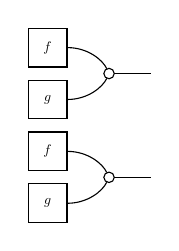
\begin{tikzpicture}[yscale=-1,x=1em,y=1.25em]
    
    \node (F1) [draw, anchor=east, minimum size=1.4em, fill=white] at (0,0) {\scalebox{0.5}{$f$}};
    \node (G1) [draw, anchor=east, minimum size=1.4em, fill=white] at (0,1.5) {\scalebox{0.5}{$g$}};
    \node (F2) [draw, anchor=east, minimum size=1.4em, fill=white] at (0,3) {\scalebox{0.5}{$f$}};
    \node (G2) [draw, anchor=east, minimum size=1.4em, fill=white] at (0,4.5) {\scalebox{0.5}{$g$}};

    \node (C1) [draw, circle, fill=white, scale=0.4] at (1.5,0.75) {};
    \node (C2) [draw, circle, fill=white, scale=0.4] at (1.5,3.75) {};

    \coordinate (O1) at (3,0.75);
    \coordinate (O2) at (3,3.75);

    \draw (F1) to[out=0, in=255] (C1);
    \draw (G1) to[out=0, in=105] (C1);
    \draw (F2) to[out=0, in=255] (C2);
    \draw (G2) to[out=0, in=105] (C2);
    \draw (C1) to (O1);
    \draw (C2) to (O2);

\end{tikzpicture}
\end{document}